\documentclass[20pt,border=5pt,transparent]{standalone}
\usepackage[english]{babel}
\usepackage[utf8]{inputenc}
\usepackage[singlelinecheck=false]{caption}
\usepackage{lipsum}
\usepackage{listings}
\usepackage{shortvrb}
\usepackage{stfloats}
\usepackage[svgnames]{xcolor}
\usepackage{tcolorbox}
\usepackage{tikz}
\tcbuselibrary{skins}
\usepackage{afterpage} % For controlling page breaks
\usepackage{ifthen} % Add the ifthen package

\captionsetup[table]{labelformat=empty,font={sf,sc,bf,},skip=0pt}
\MakeShortVerb{|}
\lstset{%
  basicstyle=\ttfamily,
  language=[LaTeX]{TeX},
  breaklines=true,
}

% Include custom command definitions and tcolorbox settings
% Custom command definitions for D&D item cards
% Add your command definitions here

\newcommand{\ItemTags}[4]{% #1=item type, #2=rarity, #3=0 for no attunement, #3=1 for attunement, #3=2 for special attunement, #4=special attunement req
    \ifnum#3=0
        \textbf{#1, #2 }\\[0.25ex]
        \\[0.25ex]
        
    \fi
    
    \ifnum#3=1
        \textbf{#1, #2 (requires attunement)}
        \\[0.25ex]
        
    \fi

    \ifnum#3=2
        \textbf{#1, #2 (requires attunement by a #4)}
        \\[0.25ex]
        
    \fi
    
    
}

\newcommand{\FlavorText}[2]{%#1=1 for flavor text, #2=flavor text
    \ifnum#1=1
        #2
        \\[0.25ex]
        
    \fi
}

\newcommand{\ChargeMechanics}[9]{% #1=total charges, #2=dice num, #3=dice sides, #4=modifier, #5=reset time, #6=1 for special charge condition, #7=special charge condition, #8=1 for last charge effect, #9=last charge effect
    \ifnum#1>1
        This item has #1 charges and regains #2d#3 + #4 expended charges daily at #5.
        \ifnum#6=1
            #7 
        \fi
        \ifnum#8=1
            #9 
        \fi
        \\[0.25ex]
        
    \fi
    \ifnum#1=1
        This item has #1 charge and regains #2d#3 + #4 expended charges daily at #5.
        \ifnum#6=1
            #7 
        \fi
        \ifnum#8=1
            #9 
        \fi
        \\[0.25ex]
        
    \fi
    
}

\newcommand{\SpellCasting}[6]{% #1=1 for spellcasting, #2=spell bonus, #3=spell bonus condition, #4=1 for additional spell effects, #5=spells, #6=additional spell effects
  \ifnum#1=1
    \textbf{Spells. }
    \ifnum#2>0
        You gain a +#2 bonus to your spell #3
    \fi
    #5
    \ifnum#4=1
        #6
    \fi
    \\[0.25ex]
    
  \fi
  
}
\newcommand{\CurseText}[2]{% #1=1 for curse, #2 for curse text
  \ifnum#1=1
    \textbf{Curse.} #2
    \\[0.25ex]
    
  \fi
}
\newcommand{\BonusText}[3]{% #1=1 for bonus text, #2 for title, #3 for text
  \ifnum#1=1
    \textbf{#2.} #3 
    \\[0.25ex]
    
  \fi
}

% \begin{itemcard}{Item Name}
%     \begin{center}
%       \begin{tcolorbox}[width=\linewidth, boxrule=3.0pt, colframe=black, colback=white, boxsep=0pt, top=0pt, bottom=0pt, left=0pt, right=0pt, center={yshift=-5mm}]
        
%         \includegraphics[width=\linewidth]{item_pics/item.png} 
%         % Replace with your image file name %
        
%       \end{tcolorbox}
%     \end{center}
%     \begin{lowerpart}
%         % Any where you see {___ Flag}, replacing it a {1} turns on that command.
        
%         % \ItemTags{Type}{Rarity}{Attunement Type}{Special Attunement Requirement}
%         % {Attunement Type} = {0}, No Attunement
%         % {Attunement Type} = {1}, Attunement
%         % {Attunement Type} = {2}, Attunement with conditions
        
%         % \FlavorText{Flavor Flag}{Flavor text placeholder}
        
%         % \ChargeMechanics{Total # of Charges}{# of Dice}{# of Sides}{Modifier}{Reset Time}{Special Recharge Flag}{Special Recharge Text}{Last Charge Effect Flag}{Last Charge Effect Text}
        
%         % \SpellCasting{Spellcasting Flag}{Spell Bonus}{Spell Bonus Condition}{Additional Effect Flag}{Spells List}{Additional Spell Effects}
%         % \BonusText{Bonus Flag}{Bonus Title}{Bonus Text}
%         % \CurseText{Curse Flag}{Curse Description}


%         \ItemTags{Type (subtype)}{rarity}{2}{creature}
%         \FlavorText{1}{You can do multiple cards of different sizes in one go in case you want to print them off.}
%         \CurseText{1}{It doesn't make separate PNGs for each item card. 
%         It also doesn't allow for giving each card a different color scheme.}
%     \end{lowerpart}
% \end{itemcard}

% \end{document}
% tcolorbox settings for D&D item cards
\newtcolorbox{itemcardauto}[2][]{
  arc=5mm,
  outer arc=5mm,
  colback=DimGray,
  colframe=black,
  boxrule=3pt,
  leftrule=3pt,
  rightrule=3pt,
  fonttitle=\large\bfseries,
  coltitle=black,
  colbacktitle=WhiteSmoke,
  enhanced,
  attach boxed title to top center={yshift=-5mm},
  boxed title style={boxrule=3pt,colframe=black, colback=WhiteSmoke,arc=5mm,outer arc=5mm},
  title=#2,
  #1
}

\newtcolorbox{lowerpartauto}[1][]{
  boxrule=3.0pt,
  colframe=black,
  coltext=black, % Black text on a black background
  enhanced,
  % sharp corners,
  borderline={0.5mm}{0mm}{black},
  #1
}

\newtcolorbox{itemcard}[2][equal height group=A, width=\cardwidth, height=\cardheight]{
  arc=5mm,
  outer arc=5mm,
  colback=DimGray,
  colframe=black,
  colbacktitle=black,
  coltitle=WhiteSmoke,
  boxrule=3pt,
  leftrule=3pt,
  rightrule=3pt,
  % sharp corners,
  fonttitle=\large\bfseries,
  enhanced,
  attach boxed title to top left={xshift=1cm,yshift*=-\tcboxedtitleheight},
  boxed title style={boxrule=1mm, frame code={
  \path[fill=tcbcolback!30!black]
  ([yshift=-1mm,xshift=-1mm]frame.north west)
  arc[start angle=0,end angle=180,radius=1mm]
  ([yshift=-1mm,xshift=1mm]frame.north east)
  arc[start angle=180,end angle=0,radius=1mm];
  \path[left color=tcbcolback!60!black,right color=tcbcolback!60!black,
  middle color=tcbcolback!80!black]
  ([xshift=-2mm]frame.north west) -- ([xshift=2mm]frame.north east)
  [rounded corners=1mm]-- ([xshift=1mm,yshift=-1mm]frame.north east)
  -- (frame.south east) -- (frame.south west)
  -- ([xshift=-1mm,yshift=-1mm]frame.north west)
  [sharp corners]-- cycle;
  },interior engine=empty,
  },
  title=#2,
  #1
}

\newtcolorbox{lowerpart}[1][height=0.425\cardheight]{
  boxrule=3.0pt,
  colframe=black,
  coltext=black, % Black text on a black background
  enhanced,
  % sharp corners,
  borderline={0.5mm}{0mm}{black},
  interior style={
    fill overzoom image=img/paper.jpg,
    fill image opacity=1,
  },
  #1
}

\newtcolorbox{backpart}[1][height=0.91625\cardheight]{
    boxrule=3.0pt,
    colframe=black,
    coltext=black, % Black text on a black background
    enhanced,
    % sharp corners,
    borderline={0.5mm}{0mm}{black},
    interior style={
    fill overzoom image=img/paper.jpg,
    fill image opacity=1,
    },
    #1
}

% By setting this option to true, you will generate a single card that scales its length to the amount of text provided. By setting it to false, you will generate a card in a 5:7 aspect ratio for printing, the same as a playing card. It will also include a card backside for overflow text.
\newboolean{autosizing}
\setboolean{autosizing}{true} 
\newlength{\cardwidth}
\newlength{\cardheight}
\setlength{\cardwidth}{5in} % Adjust the width as needed
\setlength{\cardheight}{7in} % Adjust the height as needed


\begin{document}


\ifthenelse{\boolean{autosizing}}{

    % Edit this section to change the cards meant for digital distribution. Little to no formatting should be necessary here.
    
    \begin{itemcardauto}{Item Name}
        \begin{center}
        
            % Settings for inserting item art. If you don't have any art, feel free tomment out the following tcolorbox environment. This should work with art of most sizes/ratios, but you might have to make adjustments here.
            % Included in the img folder are a number of background options. To change the background, change the referenced image in the tcolorbox interior style setting below. 
            
            \begin{tcolorbox}[width=\linewidth, boxrule=3.0pt, colframe=black,  boxsep=0pt, top=0pt, bottom=0pt, left=0pt, right=0pt, enhanced, borderline={0.5mm}{0mm}{black}, interior style={fill overzoom image=img/paper.jpg, fill image opacity=1}]
                
                % Replace with your image file name here.
                
                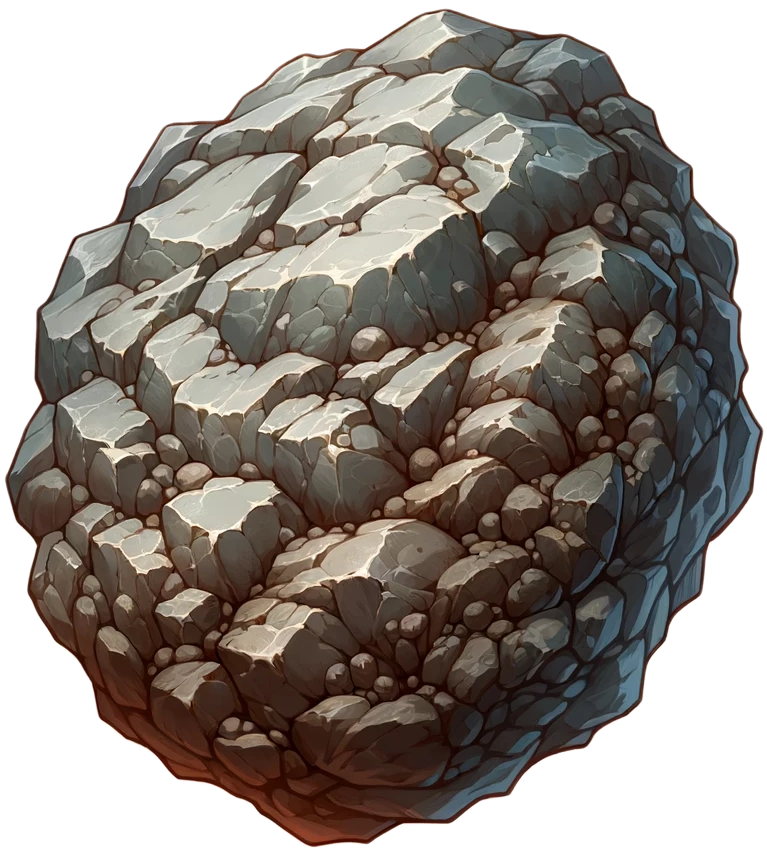
\includegraphics[width=\linewidth]{item_pics/rock_NB.png}
        
            \end{tcolorbox}
        \end{center}
        \begin{lowerpartauto}

            % Any where you see {___ Flag}, replacing it with a {1} turns on that command.
        
            % \ItemTags{Type}{Rarity}{Attunement Type}{Special Attunement Requirement}
            % {Attunement Type} = {0}, No Attunement
            % {Attunement Type} = {1}, Attunement
            % {Attunement Type} = {2}, Attunement with conditions
            
            % \FlavorText{Flavor Flag}{Flavor text}
            
            % \ChargeMechanics{Total # of Charges}{# of Dice}{# of Sides}{Modifier}{Reset Time}{Special Recharge Flag}{Special Recharge Text}{Last Charge Effect Flag}{Last Charge Effect Text}
            
            % \SpellCasting{Spellcasting Flag}{Spell Bonus}{Spell Bonus Condition}{Additional Effect Flag}{Spells List}{Additional Spell Effects}
            
            % \BonusText{Bonus Flag}{Bonus Title}{Bonus Text}
            
            % \CurseText{Curse Flag}{Curse Description}

            
            \ItemTags{Type (subtype)}{rarity}{2}{creature}
            \FlavorText{1}{This latex template allows you to create simple, automatically formatted item cards. 
            The height of the card will adjust automatically, so you don't need to worry about font sizes or having too many breaks. 
            If you want a card optimized for double-sided printing that will fit in a card sleeve, set autosizing to false. 
            
            It also makes a PNG with a transparent background. 
            If you are using this in \textbf{Overleaf}, the PNG is located in 'Logs and output files' under 'Other logs and files'. 
            To change the name of the PNG and resolution, edit the latexmkrc file.
            All of the text generating commands are defined in itemCommands.tex. 
            Card color/shape formatting is in tcolorboxSettings.tex.}
            \ChargeMechanics{1}{1}{1}{0}{thirteen o'clock}{1}{This is where you put alternative recharge mechanics, if any.}{1}{This is where you put any effect that occurs when you expend the last charge, if any.}
            \SpellCasting{1}{1}{saves and/or attack bonus, potentially with caveats.}{1}{You can use an action to expend one or more of the item's charges to cast one of the following spells at a spell save DC of 40: \textit{spell a} ($\alpha$ charges),  \textit{spell b} ($\beta$ charges), ... , \textit{spell z} ($\omega$ charges).}{Put any other spell affects the item grants here. Could be a conditional free casting of a spell on the list, extra flavor, a spell that can only be cast 1/day, etc.}
            \BonusText{1}{Extra Stuff}{If the item has other abilities/information/etc put it here.}
            \BonusText{1}{Extra Stuff 2}{The item might have multiple abilities as well, so don't be afraid to repeat this command.}
            \CurseText{1}{Always finish off with your curse, if applicable. 
            If the curse doesn't immediately reveal itself, I highly recommend making two cards: One with the curse description and one without. 
            Nothing better than handing over the "actual" item info when you player realizes something is wrong. 
            If you want to be really cheeky, change the card background color in tcolorboxSettings.tex for the cursed version to really drive it home.}
        \end{lowerpartauto}
    \end{itemcardauto}

    
    \begin{itemcardauto}{Item Name}
        \begin{center}
          \begin{tcolorbox}[width=\linewidth, boxrule=3.0pt, colframe=black,  boxsep=0pt, top=0pt, bottom=0pt, left=0pt, right=0pt, enhanced, borderline={0.5mm}{0mm}{black}, interior style={fill overzoom image=img/paper.jpg, fill image opacity=1}]
          
            % Replace with your image file name
            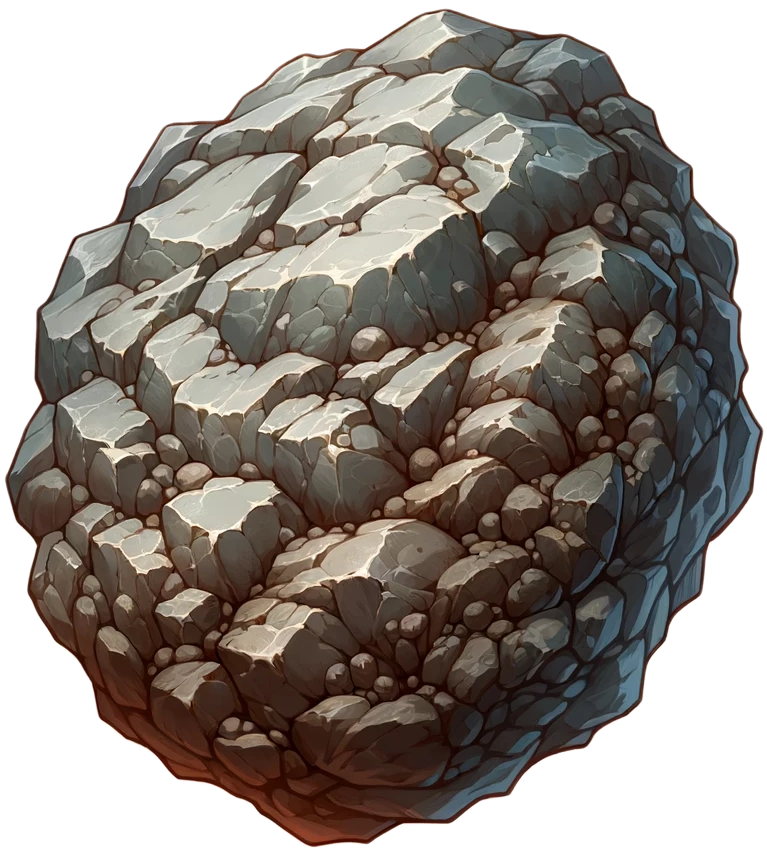
\includegraphics[width=\linewidth]{item_pics/rock_NB.png} 
            
            
          \end{tcolorbox}
        \end{center}
        \begin{lowerpartauto}
            % Any where you see {___ Flag}, replacing it a {1} turns on that command.
            
            % \ItemTags{Type}{Rarity}{Attunement Type}{Special Attunement Requirement}
            % {Attunement Type} = {0}, No Attunement
            % {Attunement Type} = {1}, Attunement
            % {Attunement Type} = {2}, Attunement with conditions
            
            % \FlavorText{Flavor Flag}{Flavor text placeholder}
            
            % \ChargeMechanics{Total # of Charges}{# of Dice}{# of Sides}{Modifier}{Reset Time}{Special Recharge Flag}{Special Recharge Text}{Last Charge Effect Flag}{Last Charge Effect Text}
            
            % \SpellCasting{Spellcasting Flag}{Spell Bonus}{Spell Bonus Condition}{Additional Effect Flag}{Spells List}{Additional Spell Effects}
            % \BonusText{Bonus Flag}{Bonus Title}{Bonus Text}
            % \CurseText{Curse Flag}{Curse Description}
    
    
            \ItemTags{Type (subtype)}{rarity}{2}{creature}
            \FlavorText{1}{You can do multiple cards of different sizes in one go in case you want to print them off in their longer form.}
            \CurseText{1}{It doesn't make separate PNGs for each item card. 
            It also doesn't allow for giving each card a different color scheme.}
        \end{lowerpartauto}
    \end{itemcardauto}
}{


    % Edit this section to change the cards meant for printed distribution. For best results, you will likely have to move text around between the front and back of the card here. 

    \begin{tikzpicture}
        \node[minimum width=\cardwidth, minimum height=\cardheight, draw, rectangle, fill=white] at (0,0) {
            \begin{itemcard}{Item Name}
                \begin{center}

                % Here is where you modify the item art. If you have a background splash you'd like to use behind your item art, put it in the interior style setting of the tcolorbox. If you want just want to use the same texture as the text boxes, use the following instead:
                % interior style={fill overzoom image=img/paper.jpg, fill image opacity=1}
                
                

                    \begin{tcolorbox}[width=\linewidth, boxrule=3.0pt, colframe=black,  boxsep=0pt, top=0pt, bottom=0pt, left=0pt, right=0pt, enhanced, borderline={0.5mm}{0mm}{black}, interior style={fill stretch image=img/ROYGBIV1.jpg}]
                        \begin{center}
                            % Place your item art here. Do not change the height, or it will mess with the card dimensions. I recommend using item art with a transparent background so that you can use the tcolorbox settings to add your backsplash.
                            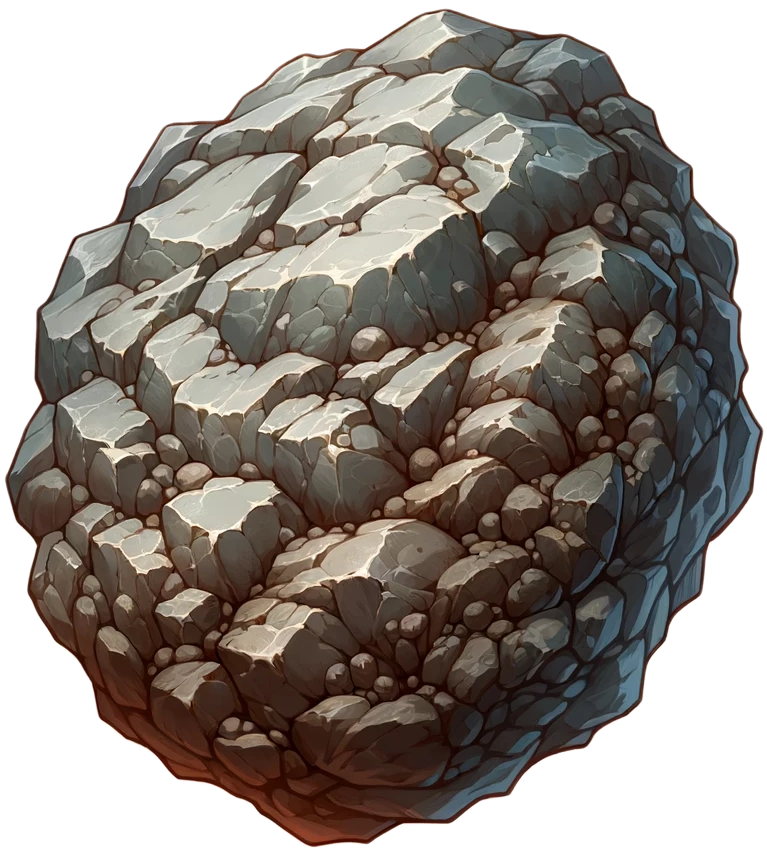
\includegraphics[height=0.455\cardheight]{item_pics/rock_NB.png}
                        \end{center}
                    \end{tcolorbox}
                \end{center}

                \begin{lowerpart}
                    % Any where you see {___ Flag}, replacing it with a {1} turns on that command.
        
                    % \ItemTags{Type}{Rarity}{Attunement Type}{Special Attunement Requirement}
                    % {Attunement Type} = {0}, No Attunement
                    % {Attunement Type} = {1}, Attunement
                    % {Attunement Type} = {2}, Attunement with conditions
                    
                    % \FlavorText{Flavor Flag}{Flavor text}

                    \ItemTags{Type (subtype)}{rarity}{2}{creature}
                    \FlavorText{1}{This latex template allows you to create simple, automatically formatted item cards. 
                    The height of the card will adjust automatically, so you don't need to worry about font sizes or having too many breaks. 
                    If you want a card optimized for double-sided printing that will fit in a card sleeve, set autosizing to false. 
                    
                    It also makes a PNG with a transparent background. 
                    If you are using this in \textbf{Overleaf}, the PNG is located in 'Logs and output files' under 'Other logs and files'. 
                    To change the name of the PNG and resolution, edit the latexmkrc file.
                    All of the text generating commands are defined in itemCommands.tex. 
                    Card color/shape formatting is in tcolorboxSettings.tex.}
                \end{lowerpart}
           \end{itemcard}
        };
    \end{tikzpicture}
    \begin{tikzpicture}
        \node[minimum width=\cardwidth, minimum height=\cardheight, draw, rectangle,fill=white] at (0,0) {
            \begin{itemcard}{Item Name}
                \begin{backpart}
                    % \ChargeMechanics{Total # of Charges}{# of Dice}{# of Sides}{Modifier}{Reset Time}{Special Recharge Flag}{Special Recharge Text}{Last Charge Effect Flag}{Last Charge Effect Text}
                    
                    % \SpellCasting{Spellcasting Flag}{Spell Bonus}{Spell Bonus Condition}{Additional Effect Flag}{Spells List}{Additional Spell Effects}
                    
                    % \BonusText{Bonus Flag}{Bonus Title}{Bonus Text}
                    
                    % \CurseText{Curse Flag}{Curse Description}
                    \ChargeMechanics{1}{1}{1}{0}{thirteen o'clock}{1}{This is where you put alternative recharge mechanics, if any.}{1}{This is where you put any effect that occurs when you expend the last charge, if any.}
                    \SpellCasting{1}{1}{saves and/or attack bonus, potentially with caveats.}{1}{You can use an action to expend one or more of the item's charges to cast one of the following spells at a spell save DC of 40: \textit{spell a} ($\alpha$ charges),  \textit{spell b} ($\beta$ charges), ... , \textit{spell z} ($\omega$ charges).}{Put any other spell affects the item grants here. Could be a conditional free casting of a spell on the list, extra flavor, a spell that can only be cast 1/day, etc.}
                    \BonusText{1}{Extra Stuff}{If the item has other abilities/information/etc put it here.}
                    \BonusText{1}{Extra Stuff 2}{The item might have multiple abilities as well, so don't be afraid to repeat this command.}
                    \CurseText{1}{Always finish off with your curse, if applicable. 
                    If the curse doesn't immediately reveal itself, I highly recommend making two cards: One with the curse description and one without. 
                    Nothing better than handing over the "actual" item info when you player realizes something is wrong. 
                    If you want to be really cheeky, change the card background color in tcolorboxSettings.tex for the cursed version to really drive it home.}
                \end{backpart}
            \end{itemcard}
        };
    \end{tikzpicture}
}




\end{document}










